\documentclass[pdf]{beamer}
% This is a LaTeX presentation template. Default themes and colours are used.
% A full list of beamer themes and colours are listed here:
% http://www.hartwork.org/beamer-theme-matrix/. To start with use the Default
% theme.

% You will need to include packages as with standard documents if you want 
% to add % features such graphics and additional mathematical symbols.
\usepackage{graphicx}

% Turn off navigation symbols.
\setbeamertemplate{navigation symbols}{}

%Create the title
\title{My first slideshow}
\author{Susan Hutchinson}
\institute{Department of Statistics, University of Oxford}
%End of title

% End of preamble
\begin{document}

% Each slides starts with \begin{frame} and ends with \end{frame}
\begin{frame}
  \titlepage % This produces the title slide
\end{frame}

\begin{frame}
\frametitle{A list} % Use frametitle for the slide title
Enter the text for your slide here.

Here is a list.
\begin{itemize}
\item One
\item Two
\item Three
\end{itemize}
\end{frame}
% End the slide

\begin{frame}
\frametitle{A list with a pause} 
 Here is another list. Note the use of  a pause between the second and third item. When giving
 the presentation you will need to hit the `enter' or `PgDn' key to display the final item.
\begin{itemize}
\item One
\item Two
\pause
\item Three
\end{itemize}
\end{frame}

\begin{frame}
\frametitle{An equation}
This is a displayed equation.

\[
\lim_{n \to \infty}
\sum_{k=1}^n \frac{1}{k^2}
= \frac{\pi^2}{6}
\]
\end{frame}

\begin{frame}
\frametitle{A plot}
Here is a plot

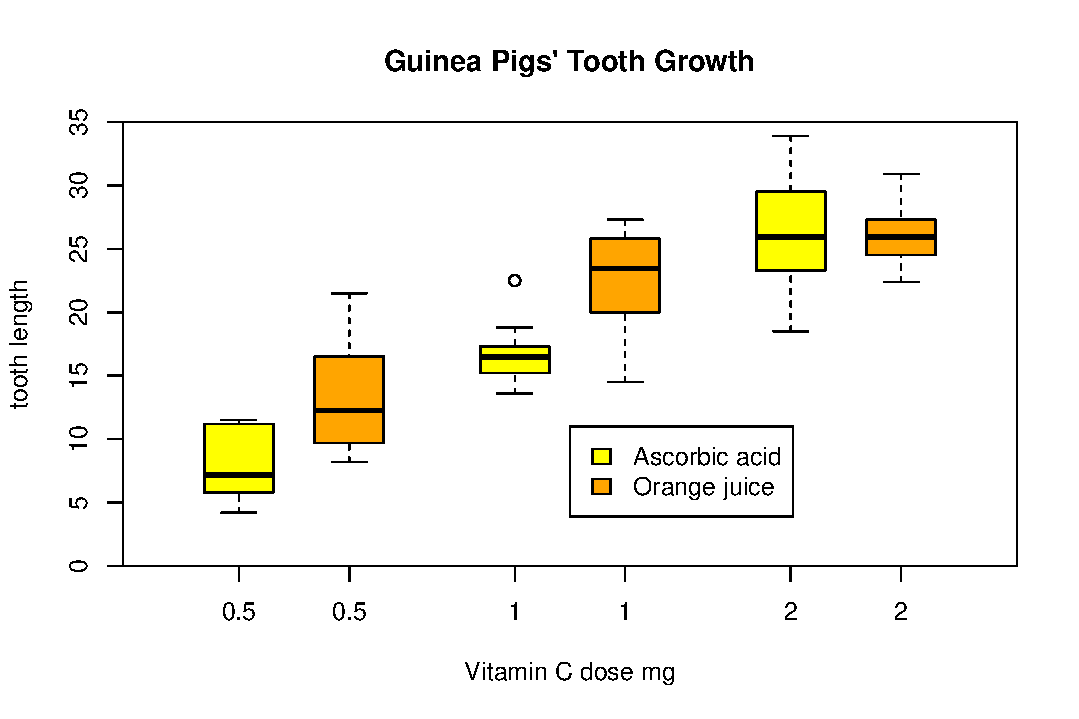
\includegraphics[width=4.8in, height=3.2in]{GuineaPigPlot.pdf}
\end{frame}

\end{document}
